In this section, I explain the data analysis, cleaning, transformation, feature engineering, and models.

\section{Cleaning pointing scan data}
\subsection{Cleaning rules}
The pointing scan data is noisy, and contains a lot of outliers.
In order to make the data more suitable for machine learning, we need to clean the data.
Below is a list of some criteria we use to filter out scans.
\begin{itemize}
    \item Scans using the HOLO transmitter.
    These scans are aiming at a radio tower, and is therefore not realistic data to train the ML model with.
    \item Scans using ZEUS2.
    These are highly experimental pointing scans and unreliable.
    \item Scans using CHAMP690, as there are very few scans using this instrument.
    \item Scans in January and February.
    There are not many scans in this time period, and the few we have involve a lot of testing.
    \item Scans that are tracking tests.
\end{itemize}   
\textcolor{red}{Find the proportion of scans that are removed from the above list.}
After this filtering, there are x out of 8862 scans left.
        
\subsection{Pointing scan classifier}
\subsubsection{Method}
In addition to the cleaning rules, we have to remove the ouright bad pointing scans (like \ref{subfig:bad_continuous} \ref{subfig:bad_line}, \ref{subfig:bad_line}).
This is done by training a classifier predict whether a scan is good or bad.
We used an XGBoost classifier with 13 features as inputs, all of which are present in the pointing scan figures (\ref{fig:line_pointings} and \ref{fig:continueous_pointings}).
The first 12 features are the amplitudes, FWHMs and pointing offsets, along with the uncertainties of these values.
The last feature is the beamsize of the telescope for the given observing frequency.\\

We had to label a training set by manually looking at pointing scans.
The size of the training set was $369$ with $270$ good and $99$ bad scans.
We did a hyperparameter search for the max depth between $1$ and $5$, number of estimators between $1$ and $80$, 
and used the \textit{scale\_pos\_weight} to consider the unbalanced classes.
The value for this parameter is the ratio of negative to positive classes.
$80\%$ of the data was used for training, and the rest for testing, which corresponds to $295$ and $74$ samples for training and testing respectively.


\begin{itemize}
    \item What hyperparameters were tuned, and what are the values.
    \item Show why it is hard to clean by only noise
    \item labeling trainig set manually, size and proportion of pos neg
    \item can choose how strict we want to be on the cleanliness
    \item precicion recall curve or mAP curve?onda
\end{itemize}

\subsubsection{Results}
The XGBoost classifier performed well a $97\%$ overall accuracy on the test set.
Figure \ref{fig:pointing_scan_clf} shows the precicion-recall curve on the left and the average precision curve on the right.
From the precision-recall curve it is clear that we can achieve a close to $100\%$ precision while still having a high recall.
This is ideal, as we want the training data for the pointing model to be as clean as possible.
We can select a large threshold, such that very few bad scans end up in the training data.
The average precicion curve shows an optimal threshold for maximizing the precision, which is about $80\%$.

\begin{figure}[H]
    \centering
    \begin{subfigure}[t]{0.49\textwidth}
        \centering
        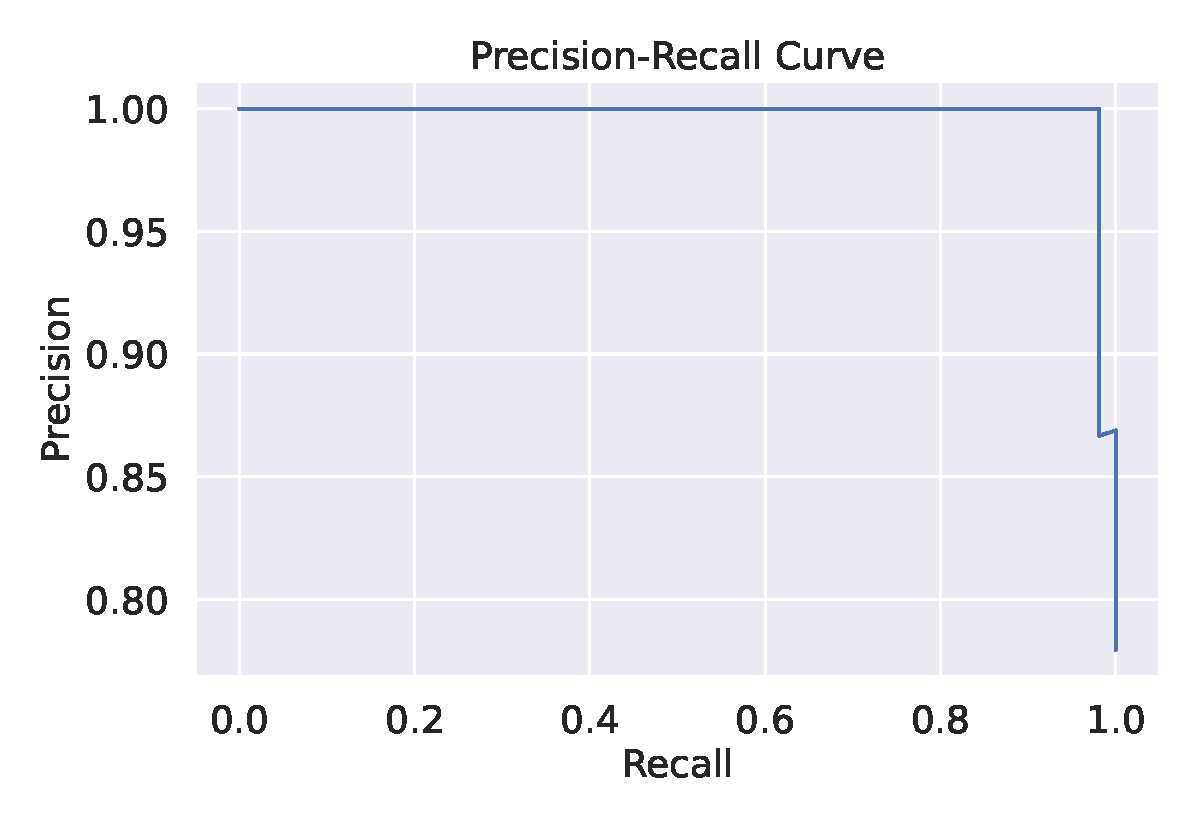
\includegraphics[width=1\textwidth]{Clf/precision_recall_curve_both.pdf}
        \caption{Precision-recall curve on test set.}
        \label{subfig:pr_curve}
    \end{subfigure}
    \begin{subfigure}[t]{0.49\textwidth}
       \centering
       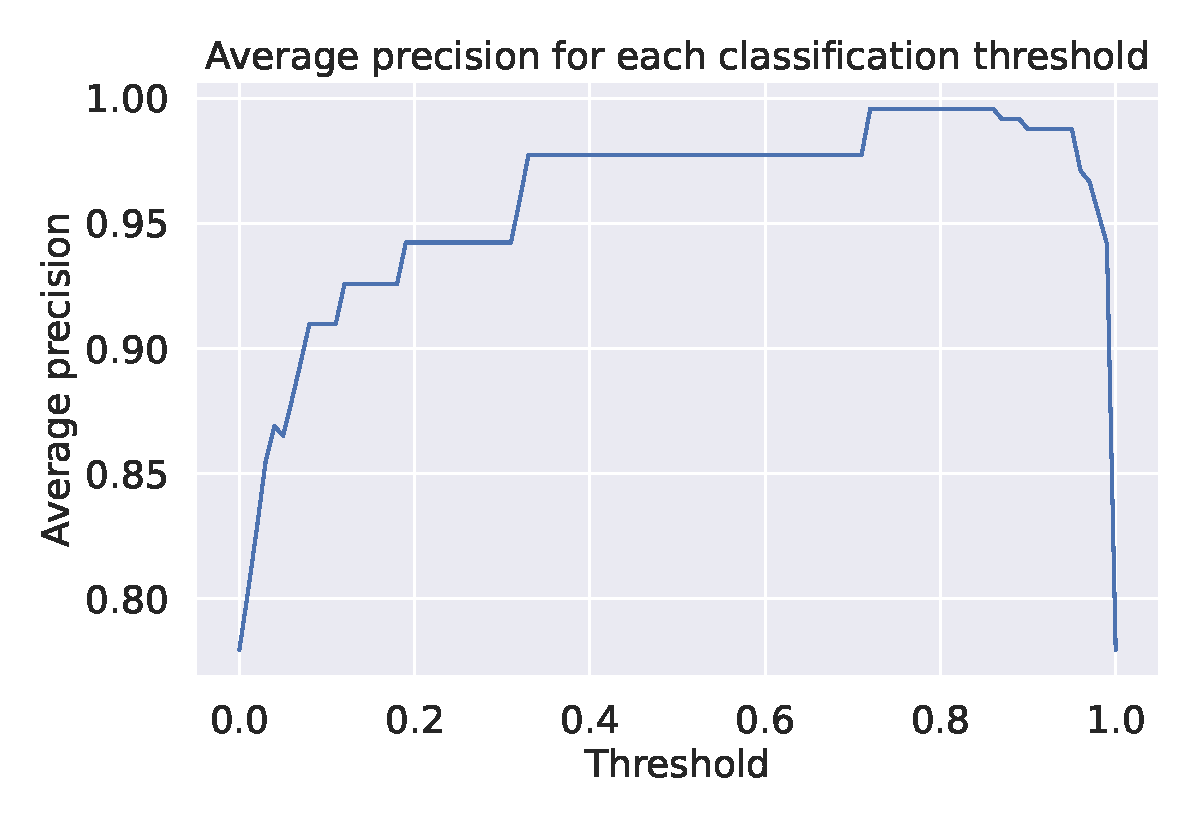
\includegraphics[width=1\textwidth]{Clf/mAP_curve_both.pdf}
       \caption{Average precision for different classification threshold.}
       \label{subfig:map_curve}
    \end{subfigure}
     \caption{Precision-recall and average precision curve for the XGBoost classifier when classifying good and bad pointing scans in the test set.}
     \label{fig:pointing_scan_clf}
\end{figure}

% \\~\\
% \begin{subfigure}[t]{0.49\textwidth}
%     \centering
%     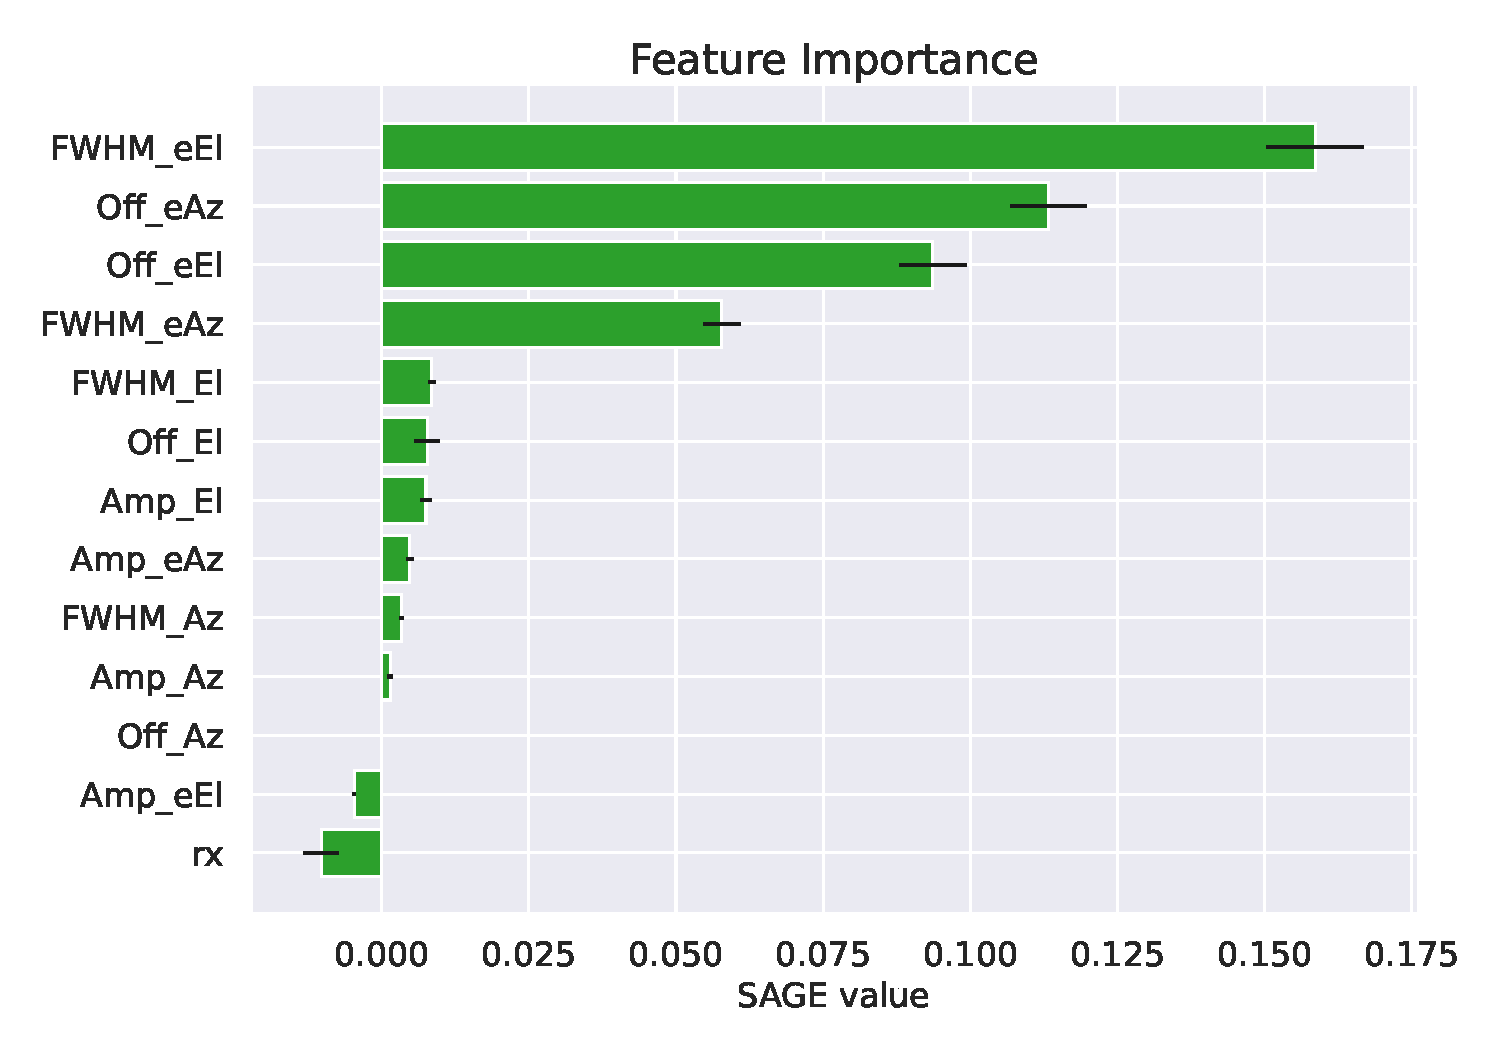
\includegraphics[width=1\textwidth]{Clf/Sage_xgb_clf_rx.pdf}
%     \caption{Average precision for different classification threshold.}
%     \label{subfig:xgb_clf_sage}
% \end{subfigure}
% \begin{figure}[H]
%     \centering
%     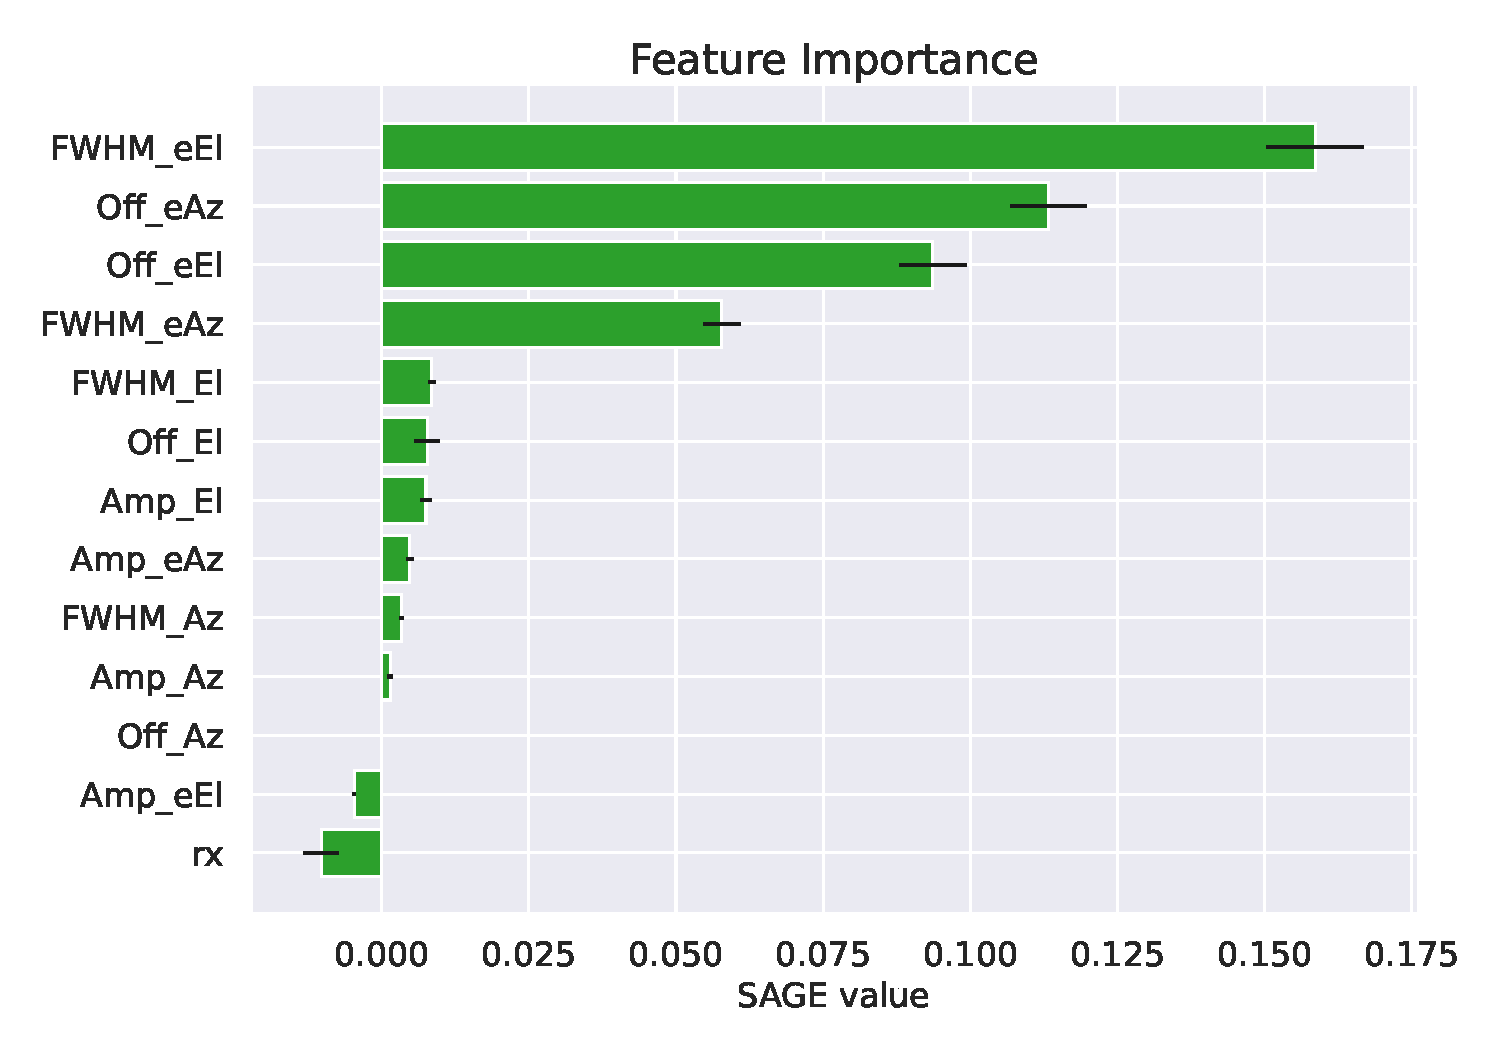
\includegraphics[width=0.98\textwidth]{Clf/Sage_xgb_clf_rx.pdf}
%     \caption{SAGE values for the XGB classifier.}
%     \label{fig:xgb_clf_sage}
% \end{figure}

\section{Scan duration analysis}
As mentioned in the database section, the timestamps of the scans is not the accurate start time of a scan.
The tiltmeter dump files with the flag indicating whether the telescope is idle, preparing to observe, or observing,
is the only data we have on when the telescope is actually performing a pointing scan.
Therefore, we need to combine the timestamp of the pointing scan with the flag in the dump files to analyse the duration of scans.

\subsection{Method}
First, we convert the different scan flags to numbers.
\textit{IDLE} and \textit{PREPARING} is the set $0$, and \textit{OBSERVING} is set to $1$.
Then we can subtract the previous rows from all rows, which will result in a value of $1$ when the scan starts, and $-1$ when it ends.
Table \ref{tab:scan_flag_difference} shows an example of the resulting table.


\begin{table}[H]
    \centering
    \begin{tabular}{cccc}
        \toprule
        Time & Flag & Flag Integer & $\Delta$ \\
        \midrule
        11:21:21 & IDLE & $0$ & $0$ \\
        11:21:22 & PREPARING & $0$ & $0$ \\
        11:21:23 & OBSERVING & $1$ & $1$ \\
        11:21:24 & OBSERVING & $1$ & $0$ \\
        11:21:25 & OBSERVING & $1$ & $0$ \\
        11:21:26 & IDLE & $0$ & $-1$ \\
        \bottomrule
    \end{tabular}
    \caption{This table shows the tiltmeter dump file containing the telescope state flag,
            and how we find the start ($\Delta = 1$) and end ($\Delta = -1$) of a scan.}
    \label{tab:scan_flag_difference}
\end{table}

By analyzing these tables for all the scans we had tiltmeter dumps for,
we see that the first \textit{OBSERVING} flag present after a scan is about $53$ \textcolor{red}{Add accurate mean and standard deviation} seconds after the scan timestamp for the vast majority of the scans.
This is shown in the right plot in figure \ref{fig:scan_times_box}, which strongly indicates that this is the starting point of a pointing scan.
In the same plot, we also see that this is fairly constant for the different instruments.
The right plot of figure \ref{fig:scan_times_date} show the time difference in seconds between the first observing flag after a scan timestamp throughout the year.
From the plot, we may conclude that this stays constant over time.\\

Now that we have found the start of a pointing scan, we look at the durations of the scans.

The left plots in figure \ref{fig:scan_times_date} and \ref{fig:scan_times_box} show the duration of the pointing scans for different instruments.
From this figure, it is clear that the duration of a pointing scan varies a lot.
This is problematic because of the fact that we only have these tiltmeter dump files for $2862/8381\approx 34\%$ of the pointing scans.


\begin{figure}[H]
    \centering
    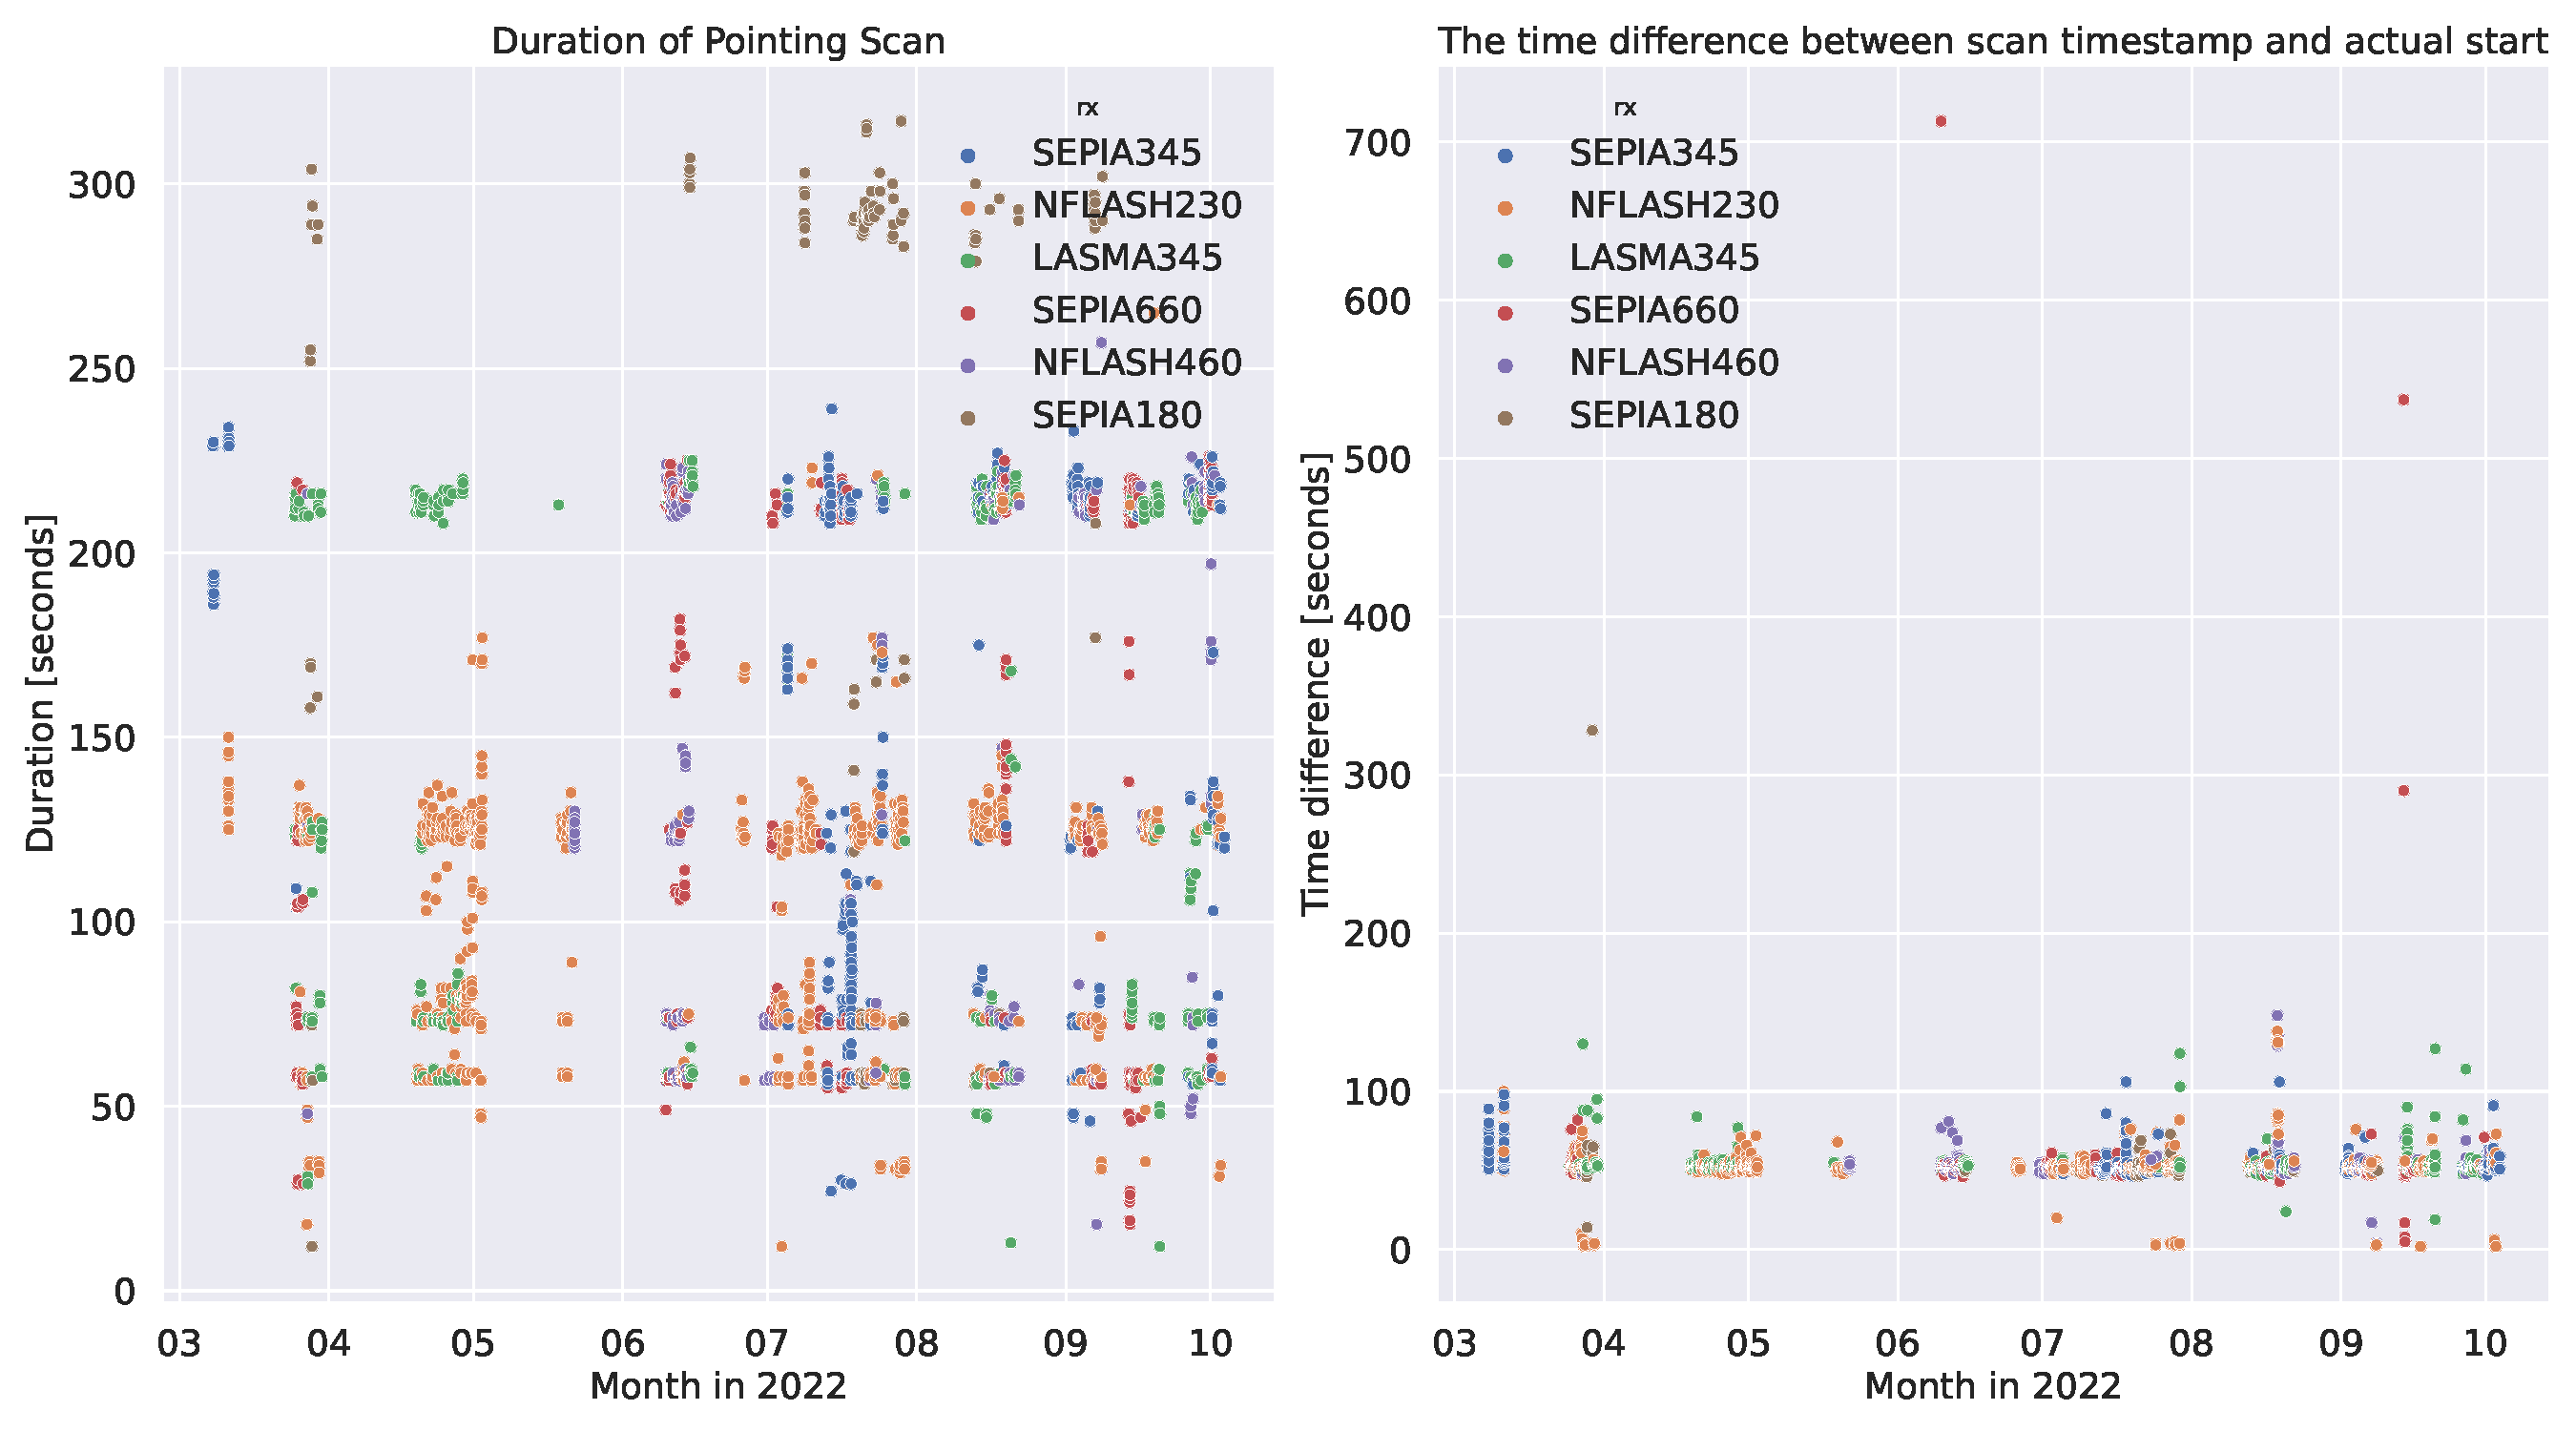
\includegraphics[width=1.1\textwidth]{Tiltmeter plots/scan_duration_distribution_date.pdf}
    \caption{Scatter plot of the duration of scans, and the time difference between the timestamp of a scan and the actual start of it.}
    \label{fig:scan_times_date}
\end{figure}

\begin{figure}[H]
    \centering
    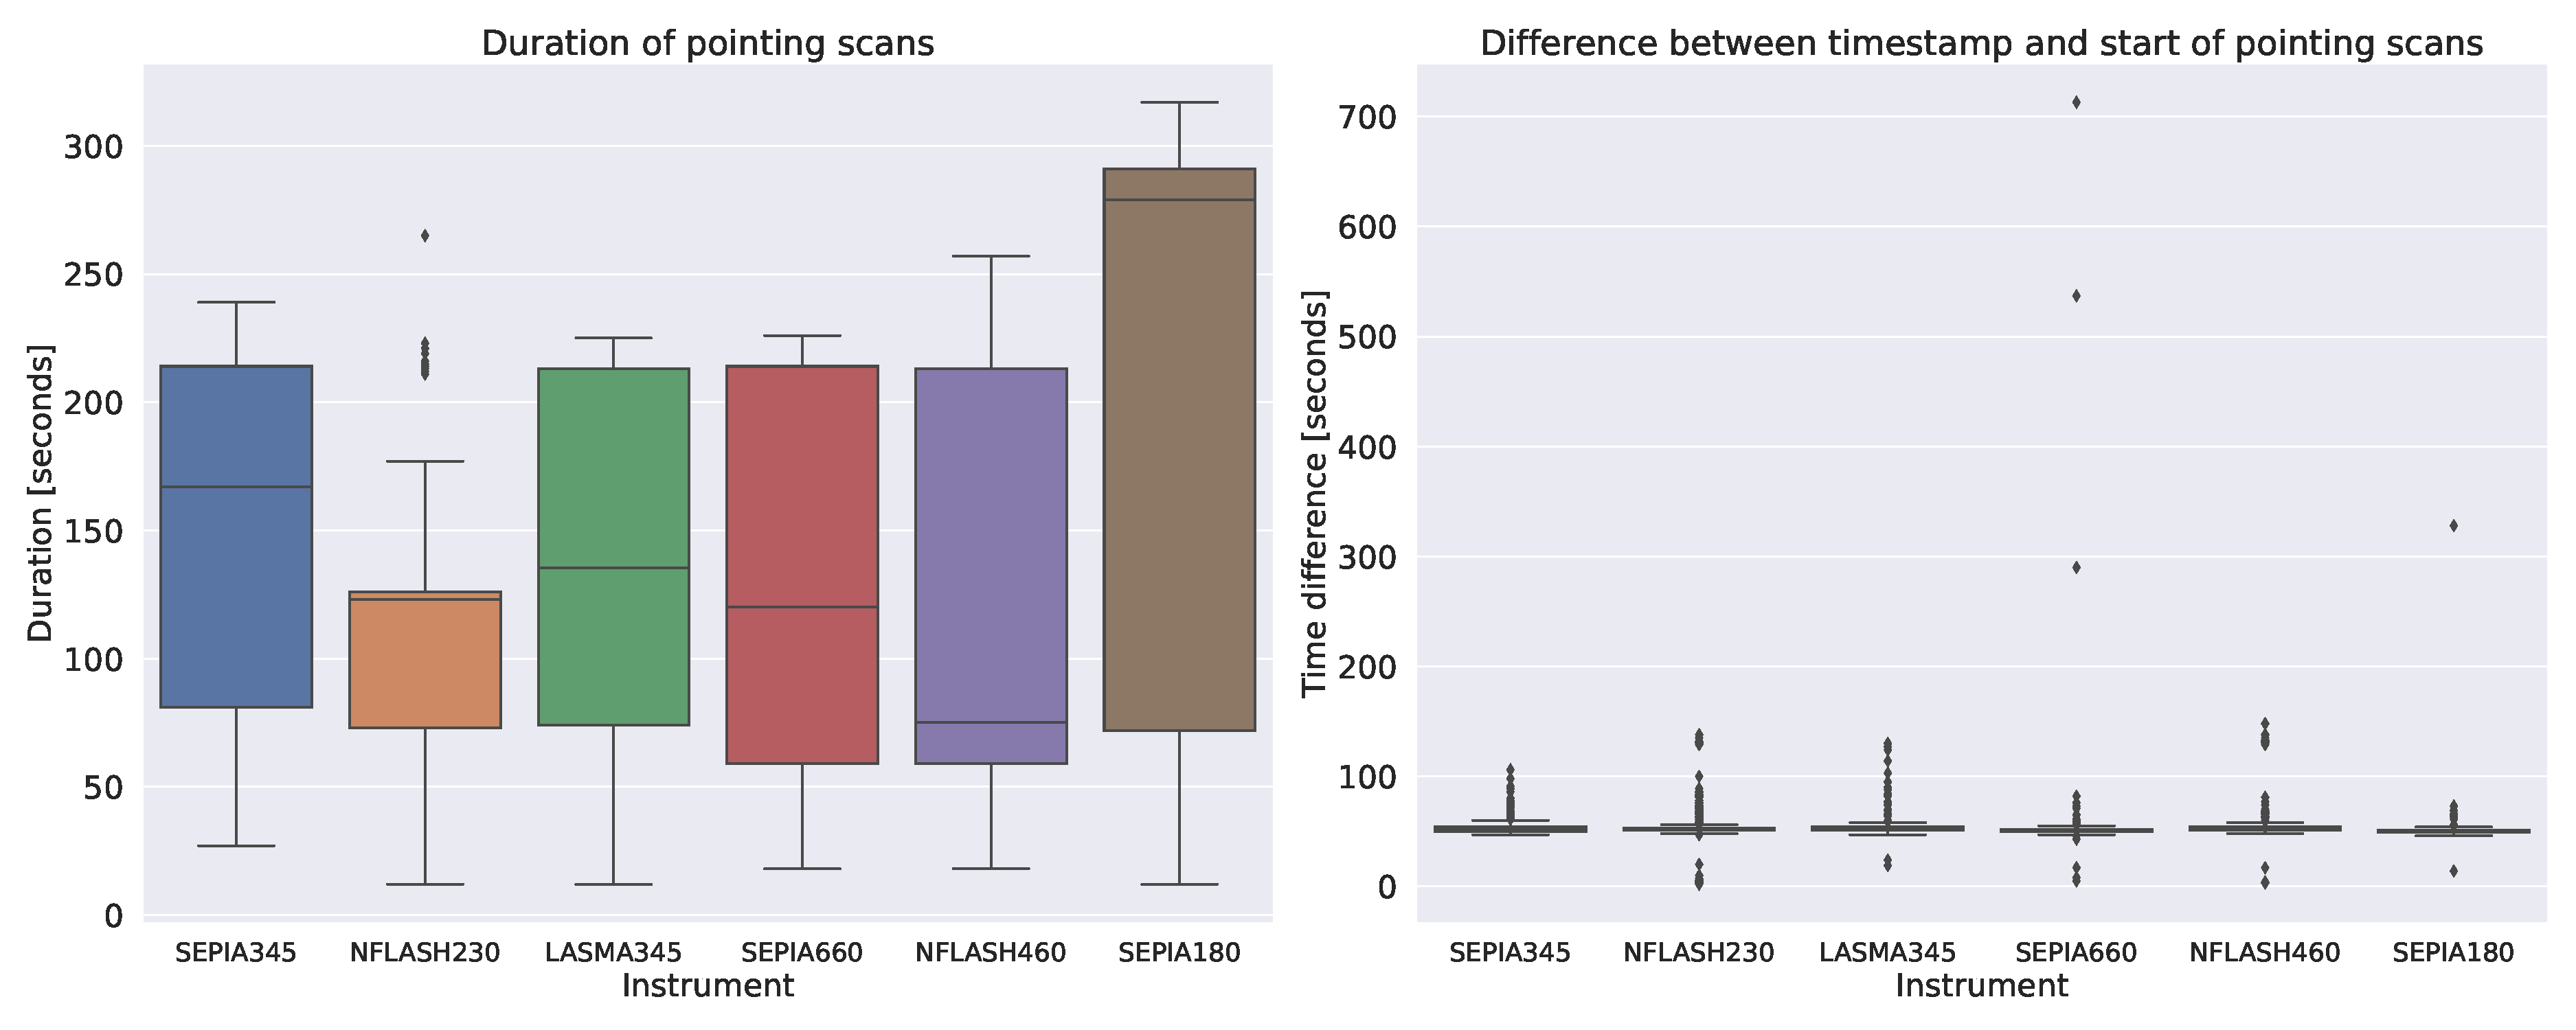
\includegraphics[width=1.1\textwidth]{Tiltmeter plots/scan_duration_distribution_rx.pdf}
    \caption{Box plot of the duration of scans, and the time difference between the timestamp of a scan and the actual start of it.}
    \label{fig:scan_times_box}
\end{figure}


\subsection{Algorithm}
Following is the algorithm used to obtain the start and end of pointing scans using the scan timestamp and the observing flag from tiltmeter dumps.

\begin{algorithm}[H]
    \caption{Find start and end of pointing scan}
    \label{alg:scan_times}
    \begin{algorithmic}
        \Require{\\
        \begin{itemize}
            \item Pointing scan timestamps $D=\{D_1,\dots,D_n\}$
            \item Timestamps $T=\{T_1,\dots,T_m\}$ and scan flag $F=\{F_1,\dots,F_m\}$
        \end{itemize}}
        \Ensure{Start and end of pointing scans $S=\{S_i,\dots,S_n\}$ and $E=\{E_i,\dots,E_n\}$}
        \For{$i=1,\dots,m$}
            \If {$F_i=OBSERVING$}
                \State {$F_i = 1$}
            \Else
                \State {$F_i = 0$}
            \EndIf
        \EndFor
        \\
        \For{$i=1,\dots,n$}
            \State {$\hat{T} = \{T_j, \text{  if  } T_j > D_i\}_j^m$}
            \State {$\hat{F} = \{F_j, \text{  if  } T_j > D_i\}_j^m$}
            \ForAll {$t_i,f_i \text{ in } \hat{T},\hat{F}$}
                \State {$\Delta = f_i-f_{i-1}$}
                \If {$\Delta = 1$}
                    \State {$S_i = t_i$}
                \EndIf
                \If {$\Delta = -1$}
                    \State {$E_i = t_i$}
                    \State {Continue}
                \EndIf
            \EndFor
        \EndFor
    \end{algorithmic}
\end{algorithm} 


\section{Feature Engineering}
\subsection{Different calculations}
There are two main types of features engineered for this project.
Features that represent the system during a pointing scan, and features that represent the changes since the last correction. 
The idea behind this is simple. The correction used during a pointing scan represents the ideal correction for the system during the previous pointing scan
As there are a lot of factors and complex relationships, and we don't have large amounts of training data, it might be easier for the model to learn 
how these changes affect the pointing rather than learning all the relationships.

\paragraph{Median values}
The median value of variables during a pointing scan is the most used feature.
Table \textcolor{red}{ref table with list of variables with median value} shows the list of variables for which we use the median values during a pointing scan.
\paragraph{Sum of all change}
To capture systematic error in pointing due to the telescope moving back and forth in azimuth and elevation,
we sum over the positive and negative changes in these variables.

Given the time of the last pointing correction $t_1$ and the start of a pointing scan $t_2$, the sum over the positive changes in a variable $x_i$ is given by
\begin{equation}\label{eq:positive_int}
    \sum_{i=t_1+1}^{t_2} \max(0, x_i-x_{i-1})
\end{equation}

Similarly, the sum of negative changes in a variable is
\begin{equation}\label{eq:negative_int}
    \sum_{i=t_1+1}^{t_2} \min(0, x_i-x_{i-1})
\end{equation}

These features are made for azimuth and elevation.

\paragraph{Change since last correction}
This feature is self-explanatory and is just the change in a variable since the pointing was corrected.
\begin{equation}
    \Delta x = x_{t_2} - x_{t_1}
\end{equation}

In order to make this feature more robust against noisy data,
we instead look at the change in the median for a time interval around the last correction $t_1$ and the start of a pointing scan $t_2$

\begin{equation}
    \Delta x = \textit{median}(x_{t_2}, x_{t_2 - 1}, \dots, x_{t_2- p}) - \textit{median}(x_{t_1}, x_{t_1 + 1}, \dots, x_{t_1 + p}),
\end{equation}
where $p$ is the number of data points needed to cover a period of $P$ minutes, given by $p = P \cdot frequency$. The unit of frequency is data points per minute, found in table \textcolor{red}{fix data freq ref}.

\paragraph{Max change in time interval}
In case the speed of the temperature change affects the deformation of the telescope's structure, we find the maximum temperature change in a given time interval since the last pointing correction.

\begin{equation}
    \max (x_{t_1+p} - x_{t_1}, x_{t_1+p} - x_{t_1}, \dots, x_{t_2} - x_{t_2-p}),
\end{equation}


\paragraph{Position of the sun}
Observers at the telescope report that the sun is affecting the pointing.
It is most drastically affected when the sun sets or rises, likely due to rapid change in temperature which leads to deformation in the telescope structure.
It is also thought that the position of the sun could play a role, and perhaps be modelled too.
For instance, if the sun is shining on the left side of the telescope, it will affect the pointing differently than if it was on the right side.
Obtaining the position of the sun for the location of the telescope is done using the python module PyEphem \cite{ephem}.

Using the azimuth angle of the sun and the telescope, we can calculate the position of the sun with respect to the pointing with
\begin{equation}\label{eq:sun_az_diff}
    \Delta \textit{Az}_\odot = \textit{Az}_{\textit{t}} - \textit{Az}_\odot
\end{equation}
This will result in values outside the $[-180^\circ,180^\circ]$. An example of this is if $Az_\odot=179^\circ$ and $Az_t = -179^\circ$.
The calculation in equation \eqref{eq:sun_az_diff} yield $-179^\circ-179^\circ=-358^\circ$,
which corresponds to the sun being $358^\circ$ to the right of the telescope, while it ideally should be $2^\circ$ to the left.
Therefore, we adjust the values accordingly
%Write equations where \Delta Az_\odot above 180 is -= 360 and under 180 is += 360
\begin{align}
    \Delta Az_\odot = Az_\odot +360^\circ, \; \text{for} \; \Delta Az_\odot < 180^\circ\\
    \Delta Az_\odot = Az_\odot -360^\circ, \; \text{for} \; \Delta Az_\odot > 180^\circ
\end{align}

Here, the interval of the difference in azimuth is fixed to the interval $(-180^\circ,180^\circ)$,
where $0^\circ$ means the telescope is pointing towards the sun in the azimuth direction.
$\Delta \textit{Az}_\odot = 90^\circ$ corresponds to the sun being direct to the left of the pointing direction. \\

Another measure tested is the total angle between the pointing and the position of the sun. This is calculated using the following formula
\begin{equation}
    \theta = \cos \textit{Az}_t \cdot \cos \textit{El}_t\cdot \cos \textit{Az}_\odot \cdot \cos \textit{El}_\odot + \sin \textit{Az}_t \cdot \cos \textit{El}_t\cdot \sin \textit{Az}_\odot \cdot \cos \textit{El}_\odot + \sin \textit{El}_t \cdot \sin \textit{El}_\odot
\end{equation}

\subsection{List of features}
\textcolor{red}{add a list of all features for different calculations here}

\section{Transformation of pointing offsets and corrections}
Table \ref{tab:offset_and_correction} shows some observed pointing offsets and the corrections applied during the pointing scan.
The pointing corrections $ca$ and $ie$ are sometimes updated according to equation \eqref{eq:ca} and \eqref{eq:ie},
as we see in the first two rows. Sometimes the corrections are not updated, like in the consecutive row. Other times, the corrections are updated, but not according to the equation \eqref{eq:ca} and \eqref{eq:ie}.
This introduces a couple of challenges for the training of a model.
\begin{itemize}
    \item $ca$ and $ie$ should represent the optimal correction using all the information we have about the current state of a system.
    If we don't update the corrections, there is some information about the system (the previously observed pointing offset) the model is not receiving.
    \item Some of the features are constructed by looking at the change in variables since the last correction.
    If the corrections are not updated, this interval is longer and the resulting features could be more prone to uncertainties and noise.
    A problem with the integration also occurs if the corrections are not updated according to the equations \eqref{eq:ca} and \eqref{eq:ie}.
    Then we don't know at what time those corrections represent the system, resulting in inaccurate features.
\end{itemize}


The following is a possible solution to these problems.
\begin{enumerate}
    \item Transform the offsets and corrections such that they represent the system at the most recent pointing scan.
    \item Use these transformed offsets as new training labels, and transformed corrections as training inputs.
\end{enumerate}

The way I do this is by assuming the corrections $ca$ and $ie$ are updated after every pointing scan.
This will change the observed pointing offsets, which again will affect the corrections during the next pointing scan.
The effects of this followed throughout the whole dataset
The following formulas 
\begin{align}
    \Tilde{ca}_i &= \Tilde{ca}_{i-1} + \Tilde{\delta}_{az,i-1}\label{eq:ca_tilde}\\
    \Tilde{ie}_i &= \Tilde{ie}_{i-1} - \Tilde{\delta}_{el,i-1\label{eq:ie_tilde}}\\
    \Tilde{\delta}_{az,i} &= \delta_{az,i} + ca_i - \Tilde{ca}_i\label{eq:off_az_tilde}\\
    \Tilde{\delta}_{el,i} &= \delta_{el,i} - ie_i + \Tilde{ie}_i\label{eq:off_el_tilde}
\end{align}
Where the "$\sim$" denotes a transformed variable.
Using these transformations,
the corrections used for training and the resulting offset are alike the ones that would be observed if the corrections were made according to the equations
\eqref{eq:ca} and \eqref{eq:ie} after every pointing scan.


\begin{table}[H]
    \centering
    \caption{Example from the dataset of the observed pointing offsets and the corrections applied during the pointing scan.}
    \label{tab:offset_and_correction}
    \begin{tabular}{ccccc}
    \toprule
    $i$ &  $\delta_{az}$ &  $\delta_{el}$ &  $ca$ & $ie$  \\
    \midrule
    1 & 1.2 & 0.1 & 2.1 &  1.7 \\
    2 &     0.0 & 0.5 & 3.3 &  1.6 \\
    3 &    -1.1 & 0.0 & 3.3 &  1.6 \\
    4 &     0.6 & 0.7 & 2.2 &  1.6 \\
    5 &     0.9 & 1.4 & 2.2 &  1.6 \\
    6 &     1.0 & 1.1 & 2.2 &  1.6 \\
    7 &    -0.9 & 1.2 & 3.1 &  0.5 \\
    8 &     0.5 & 1.5 & 2.2 & -0.7 \\
    9 &    -0.3 & 0.4 & 2.2 & -0.7 \\
    \bottomrule
    \end{tabular}
\end{table}


\begin{table}[H]
    \centering
    \caption{Table of transformed pointing offsets and corrections according to equations \eqref{eq:ca_tilde}, \eqref{eq:ie_tilde}, \eqref{eq:off_az_tilde}, and \eqref{eq:off_el_tilde}.}
    \label{tab:tranform_offsets}
\begin{tabular}{ccccc}
\toprule
$i$ & $\Tilde{\delta}_{az}$ &  $\Tilde{\delta}_{el}$ &  $\Tilde{ca}$ &  $\Tilde{ie}$ \\
\midrule
0 &       1.2 &       0.1 &       2.1 &       1.7 \\
1 &       0.0 &       0.5 &       3.3 &       1.6 \\
2 &      -1.1 &      -0.5 &       3.3 &       1.1 \\
3 &       0.7 &       0.7 &       2.2 &       1.6 \\
4 &       0.2 &       0.7 &       2.8 &       0.9 \\
5 &       0.1 &      -0.3 &       3.1 &       0.2 \\
6 &      -1.0 &       1.3 &       3.2 &       0.5 \\
7 &       0.5 &       1.4 &       2.2 &      -0.7 \\
8 &      -0.8 &      -1.1 &       2.7 &      -2.2 \\
\bottomrule
\end{tabular}
\end{table}


\section{Machine Learning Experiments}
In this section, I will provide an overview of two machine learning experiments that are pertinent to the two research questions.
The first experiment aims to investigate the effectiveness of neural networks in developing a pointing model that could potentially replace the current linear model, which is created through linear regression.
The purpose of this experiment is to explore the feasibility of a more sophisticated model in terms of pointing accuracy.
The second experiment aims to examine the effectiveness of an XGBoost model in predicting pointing scan offsets to enhance the pointing accuracy.
The primary objective of this experiment is to assess whether the proposed model can outperform the current model in terms of pointing accuracy.

\section{Experiment 1: Pointing Model using Neural Networks}
This experiment uses the raw dataset containing input coordinates, $Az_{\text{input}}$ and $El_{\text{input}}$ respectively, and corresponding true observed values $Az_{\text{observed}}$ and $El_{\text{observed}}$.

The goal is to find a model $f$ such that
\begin{equation}
    f(X) \approx (\delta_{\text{Az}}, \delta_{\text{El}}) = (Az_{\text{observed}}-Az_{\text{input}}, El_{\text{observed}}-El_{\text{input}})
\end{equation}

The dataset is split in three parts. A train, validation, and test set.
The last $15\%$ of the data, which is sorted by date, is used for testing.
The remaining $85\%$ of the data is used for training and validation, and this set is split into $20\%$ for training and $80\%$ for validation.
This results in $\approx 76\%$ and $\approx 24\%$ of the total dataset being used for training and validation respectively.


\subsection{Feature Selection}
Selecting the right features plays an important role in improving the accuracy of the pointing model.
This model uses two types of features: geometrical and harmonic terms that are already part of the current linear base model, and new features that are extracted from the telescope's database.
We identified relevant features by calculating Pearson's and Spearman's rank correlation for all features in relation to the offsets.
We analyzed the correlation of harmonic terms using sine and cosine functions of azimuth and elevation up to the fifth order, as well as the geometrical terms.
Then, we chose the terms that had the strongest correlation for the model and used them in all models.
For the features extracted from the database, we made a list of the ones that showed a correlation equal to or greater than 0.1.
During model training, we randomly selected a subset of 2 to 19 features from this list and used them to train the model.

\subsection{Model Architecture}
This experiment utilized four different model architectures.
The first architecture involved feeding all of the input data into one, two, or three hidden layers.
The other three architectures incorporated machine learning techniques by separating the geometrical and harmonic terms of the input data from the other features and processing them using distinct architectures.
These approaches were intended to keep the current model's simplicity and performance, while still incorporating new features.

The following are the four different architectures:
\begin{enumerate}
    \item \textbf{Neural Network with Separated Features 1:} This architecture separates the input features into two groups: geometric and harmonic features, and the rest of the features.
    The geometric and harmonic features are connected directly to the output layer, while the remaining features are passed through layers with non-linear activation functions.
    \item \textbf{Neural Network with Separated Features 2:} This architecture is similar to the previous architecture,
    but the geometric and harmonic features are passed through an additional layer of non-linear activation function before connecting them to the output layer.
    \item \textbf{Neural Network with Separated Features 3:} This architecture combines the previous two architectures by passing the regular features through a few hidden layers with non-linear activation functions before concatenating them with the geometric and harmonic features.
    The combined features are then passed through a final layer before connecting to the output layer.
    \item \textbf{Regular Neural Network:} All features are passed through the same layers, all with a nonlinear activation function.
\end{enumerate}
These are visualized in figure \ref{fig:nn_architecture}.

\begin{figure}[H]
    \centering
    \begin{subfigure}[t]{0.49\textwidth}
        \centering
        % NEURAL NETWORK no text - large
\begin{tikzpicture}[x=2.3cm,y=1.0cm]
  \message{^^JNeural network large}
  \readlist\Nnod{3,4,4,2} % array of number of nodes per layer
  
  \message{^^J  Layer}
  \foreachitem \N \in \Nnod{ % loop over layers
    \def\lay{\Ncnt} % alias of index of current layer
    \pgfmathsetmacro\prev{int(\Ncnt-1)} % number of previous layer
    \message{\lay,}
    \foreach \i [evaluate={\y=\N/2-\i; \x=\lay*0.8; \n=\nstyle;
                           \nprev=int(\prev<\Nnodlen?min(2,\prev):3);}] in {1,...,\N}{ % loop over nodes
      
      % NODES
      %\node[node \n,outer sep=0.6,minimum size=18] (N\lay-\i) at (\x,\y) {};
      \coordinate (N\lay-\i) at (\x,\y);
      
      % CONNECTIONS
      \ifnum\lay>1 % connect to previous layer
        \foreach \j in {1,...,\Nnod[\prev]}{ % loop over nodes in previous layer
          \draw[connect,white,line width=1.2] (N\prev-\j) -- (N\lay-\i);
          \draw[connect] (N\prev-\j) -- (N\lay-\i);
          %\draw[connect] (N\prev-\j.0) -- (N\lay-\i.180); % connect to left
          \node[node \nprev,minimum size=18] at (N\prev-\j) {}; % draw node over lines
        }
        \ifnum \lay=\Nnodlen % draw last node over lines
          \node[node \n,minimum size=18] at (N\lay-\i) {};
        \fi
      \fi % else: nothing to connect first layer
      
    }
  }
  
\end{tikzpicture}
        \caption{\textbf{Regular neural network:}
        This is the standard neural network architecture without any feature separation.
        All features are connected to the same layers.}
        \label{subfig:cm_dt}
    \end{subfigure}
    \hfill
   \begin{subfigure}[t]{0.49\textwidth}
       \centering
       \begin{tikzpicture}[x=2.3cm,y=2.0cm]
  \message{^^JNeural network large}
  \readlist\Nnod{3,2} % array of number of nodes per layer
  \readlist\Nnodtwo{2,3,3,2}
  \message{^^J  Layer}
  \foreachitem \N \in \Nnod{ % loop over layers
    \def\lay{\Ncnt} % alias of index of current layer
    \pgfmathsetmacro\prev{int(\Ncnt-1)} % number of previous layer
    \message{\lay,}
    \foreach \i [evaluate={\y=\N/4-\i*0.5; \x=\lay*0.8+1.6; \n=\nstyle;
                           \nprev=int(\prev<\Nnodlen?min(2,\prev):3);}] in {1,...,\N}{ % loop over nodes
      
      % NODES
      %\node[node \n,outer sep=0.6,minimum size=18] (N\lay-\i) at (\x,\y) {};
      \ifnum \lay<\Nnodlen % draw last node over lines
        \coordinate (N\lay-\i) at (\x,\y);
      \else
        \coordinate (N\lay-\i) at (\x,\y-0.75);
      \fi
      % CONNECTIONS
      \ifnum\lay>1 % connect to previous layer
        \foreach \j in {1,...,\Nnod[\prev]}{ % loop over nodes in previous layer
          \draw[connect,white,line width=1.2] (N\prev-\j) -- (N\lay-\i);
          \draw[connect] (N\prev-\j) -- (N\lay-\i);
          %\draw[connect] (N\prev-\j.0) -- (N\lay-\i.180); % connect to left
          \node[node \nprev,minimum size=18] at (N\prev-\j) {}; % draw node over lines
        }
        \ifnum \lay=\Nnodlen % draw last node over lines
          \node[node \n,minimum size=18] at (N\lay-\i) {};
        \fi
      \fi % else: nothing to connect first layer
      
    }
  }

  \foreachitem \N \in \Nnodtwo{ % loop over layers
    \def\lay{\Ncnt} % alias of index of current layer
    \pgfmathsetmacro\prev{int(\Ncnt-1)} % number of previous layer
    \message{\lay,}
    \foreach \i [evaluate={\y=\N/4-\i*0.5-1.5; \x=\lay*0.8; \n=\nstyle;
                           \nprev=int(\prev<\Nnodtwolen?min(2,\prev):3);}] in {1,...,\N}{ % loop over nodes
      % NODES
      %\node[node \n,outer sep=0.6,minimum size=18] (N\lay-\i) at (\x,\y) {};
      \ifnum \lay<\Nnodtwolen % draw last node over lines
        \coordinate (M\lay-\i) at (\x,\y);
      \else
        \coordinate (M\lay-\i) at (\x,\y+0.75);
      \fi
      % CONNECTIONS
      \ifnum\lay>1 % connect to previous layer
        \foreach \j in {1,...,\Nnodtwo[\prev]}{ % loop over nodes in previous layer
          \draw[connect,white,line width=1.2] (M\prev-\j) -- (M\lay-\i);
          \draw[connect] (M\prev-\j) -- (M\lay-\i);
          %\draw[connect] (N\prev-\j.0) -- (N\lay-\i.180); % connect to left
          \node[node \nprev,minimum size=18] at (M\prev-\j) {}; % draw node over lines
        }
        \ifnum \lay=\Nnodtwolen % draw last node over lines
          \node[node \n,minimum size=18] at (M\lay-\i) {};
        \fi
      \fi % else: nothing to connect first layer
      
    }
  }
  
\end{tikzpicture}
       \caption{\textbf{Neural network with separated features 1:}
       In this architecture, the geometric and harmonic features are separated from the other features and directly connected to the output layer, without any nonlinear activation function.}
       \label{subfig:cm_rf}
\end{subfigure}
\\~\\
    \begin{subfigure}[t]{0.49\textwidth}
        \centering
        \begin{tikzpicture}[x=2.3cm,y=2.0cm]
  \message{^^JNeural network large}
  \readlist\Nnod{3,3,2} % array of number of nodes per layer
  \readlist\Nnodtwo{2,3,3,2}
  \message{^^J  Layer}
  \foreachitem \N \in \Nnod{ % loop over layers
    \def\lay{\Ncnt} % alias of index of current layer
    \pgfmathsetmacro\prev{int(\Ncnt-1)} % number of previous layer
    \message{\lay,}
    \foreach \i [evaluate={\y=\N/4-\i*0.5; \x=\lay*0.8+0.8; \n=\nstyle;
                           \nprev=int(\prev<\Nnodlen?min(2,\prev):3);}] in {1,...,\N}{ % loop over nodes
      
      % NODES
      %\node[node \n,outer sep=0.6,minimum size=18] (N\lay-\i) at (\x,\y) {};
      \ifnum \lay<\Nnodlen % draw last node over lines
        \coordinate (N\lay-\i) at (\x,\y);
      \else
        \coordinate (N\lay-\i) at (\x,\y-0.75);
      \fi
      % CONNECTIONS
      \ifnum\lay>1 % connect to previous layer
        \foreach \j in {1,...,\Nnod[\prev]}{ % loop over nodes in previous layer
          \draw[connect,white,line width=1.2] (N\prev-\j) -- (N\lay-\i);
          \draw[connect] (N\prev-\j) -- (N\lay-\i);
          %\draw[connect] (N\prev-\j.0) -- (N\lay-\i.180); % connect to left
          \node[node \nprev,minimum size=18] at (N\prev-\j) {}; % draw node over lines
        }
        \ifnum \lay=\Nnodlen % draw last node over lines
          \node[node \n,minimum size=18] at (N\lay-\i) {};
        \fi
      \fi % else: nothing to connect first layer
      
    }
  }
  \node[shift = {(-1.5,0)}] at (N2-2){
    $\begin{aligned}
      \text{Geom}&\text{etric}\\
      +&\\
      \text{Harm}&\text{onics}
    \end{aligned}$
  };
  \node[shift = {(-1.5,-0.85)}] at (N2-2){Nonlinear};
  \foreachitem \N \in \Nnodtwo{ % loop over layers
    \def\lay{\Ncnt} % alias of index of current layer
    \pgfmathsetmacro\prev{int(\Ncnt-1)} % number of previous layer
    \message{\lay,}
    \foreach \i [evaluate={\y=\N/4-\i*0.5-1.5; \x=\lay*0.8; \n=\nstyle;
                           \nprev=int(\prev<\Nnodtwolen?min(2,\prev):3);}] in {1,...,\N}{ % loop over nodes
      % NODES
      %\node[node \n,outer sep=0.6,minimum size=18] (N\lay-\i) at (\x,\y) {};
      \ifnum \lay<\Nnodtwolen % draw last node over lines
        \coordinate (M\lay-\i) at (\x,\y);
      \else
        \coordinate (M\lay-\i) at (\x,\y+0.75);
      \fi
      % CONNECTIONS
      \ifnum\lay>1 % connect to previous layer
        \foreach \j in {1,...,\Nnodtwo[\prev]}{ % loop over nodes in previous layer
          \draw[connect,white,line width=1.2] (M\prev-\j) -- (M\lay-\i);
          \draw[connect] (M\prev-\j) -- (M\lay-\i);
          %\draw[connect] (N\prev-\j.0) -- (N\lay-\i.180); % connect to left
          \node[node \nprev,minimum size=18] at (M\prev-\j) {}; % draw node over lines
        }
        \ifnum \lay=\Nnodtwolen % draw last node over lines
          \node[node \n,minimum size=18] at (M\lay-\i) {};
        \fi
      \fi % else: nothing to connect first layer
      
    }
  }
  
\end{tikzpicture}
        \caption{\textbf{Neural network with separated features 2}:
        Similar to the previous architecture, the geometric and harmonic features are separated from the other features,
        but they are also processed by a nonlinear activation function before being connected to the output layer.}
        \label{subfig:cm_bag}
    \end{subfigure}
    \hfill
       \begin{subfigure}[t]{0.49\textwidth}
        \centering
        \begin{tikzpicture}[x=2.3cm,y=2.0cm]
  \message{^^JNeural network large}
  \readlist\Nnod{3,3,2} % array of number of nodes per layer
  \readlist\Nnodtwo{2,3,3,2}
  \message{^^J  Layer}
  \foreachitem \N \in \Nnod{ % loop over layers
    \def\lay{\Ncnt} % alias of index of current layer
    \pgfmathsetmacro\prev{int(\Ncnt-1)} % number of previous layer
    \message{\lay,}
    \foreach \i [evaluate={\y=\N/4-\i*0.5; \x=\lay*0.8+0.8; \n=\nstyle;
                           \nprev=int(\prev<\Nnodlen?min(2,\prev):3);}] in {1,...,\N}{ % loop over nodes
      
      % NODES
      %\node[node \n,outer sep=0.6,minimum size=18] (N\lay-\i) at (\x,\y) {};
      \ifnum \lay<\Nnodlen % draw last node over lines
        \coordinate (N\lay-\i) at (\x,\y);
      \else
        \coordinate (N\lay-\i) at (\x,\y-0.75);
      \fi
      % CONNECTIONS
      \ifnum\lay>1 % connect to previous layer
        \foreach \j in {1,...,\Nnod[\prev]}{ % loop over nodes in previous layer
          \draw[connect,white,line width=1.2] (N\prev-\j) -- (N\lay-\i);
          \draw[connect] (N\prev-\j) -- (N\lay-\i);
          %\draw[connect] (N\prev-\j.0) -- (N\lay-\i.180); % connect to left
          \node[node \nprev,minimum size=18] at (N\prev-\j) {}; % draw node over lines
        }
        \ifnum \lay=\Nnodlen % draw last node over lines
          \node[node \n,minimum size=18] at (N\lay-\i) {};
        \fi
      \fi % else: nothing to connect first layer
      
    }
  }

  \foreachitem \N \in \Nnodtwo{ % loop over layers
    \def\lay{\Ncnt} % alias of index of current layer
    \pgfmathsetmacro\prev{int(\Ncnt-1)} % number of previous layer
    \message{\lay,}
    \foreach \i [evaluate={\y=\N/4-\i*0.5-1.5; \x=\lay*0.8; \n=\nstyle;
                           \nprev=int(\prev<\Nnodtwolen?min(2,\prev):3);}] in {1,...,\N}{ % loop over nodes
      % NODES
      %\node[node \n,outer sep=0.6,minimum size=18] (N\lay-\i) at (\x,\y) {};
      \ifnum \lay<\Nnodtwolen % draw last node over lines
        \coordinate (M\lay-\i) at (\x,\y);
      \else
        \coordinate (M\lay-\i) at (\x,\y+0.75);
      \fi
      % CONNECTIONS
      \ifnum\lay>1 % connect to previous layer
        \foreach \j in {1,...,\Nnodtwo[\prev]}{ % loop over nodes in previous layer
          \draw[connect,white,line width=1.2] (M\prev-\j) -- (M\lay-\i);
          \draw[connect] (M\prev-\j) -- (M\lay-\i);
          %\draw[connect] (N\prev-\j.0) -- (N\lay-\i.180); % connect to left
          \node[node \nprev,minimum size=18] at (M\prev-\j) {}; % draw node over lines
        }
        \ifnum \lay=\Nnodtwolen % draw last node over lines
          \node[node \n,minimum size=18] at (M\lay-\i) {};
        \fi
      \fi % else: nothing to connect first layer
      
    }
  }

  \foreachitem \N \in \Nnod{ % loop over layers
    \def\lay{\Ncnt} % alias of index of current layer
    \pgfmathsetmacro\prev{int(\Ncnt-1)} % number of previous layer
    \message{\lay,}
    \foreach \i [evaluate={\y=\N-\i*0.5; \x=\lay; \n=\nstyle;
                           \nprev=int(\prev<\Nnodlen?min(2,\prev):3);}] in {1,...,\N}{ % loop over nodes
      
      % CONNECTIONS
      \ifnum\lay=2 % connect to previous layer
        \foreach \j in {1,...,\Nnod[\prev]}{ % loop over nodes in previous layer
          \draw[connect,white,line width=1.2] (M3-\j) -- (N\lay-\i);
          \draw[connect] (M3-\j) -- (N\lay-\i);
          %\draw[connect] (N\prev-\j.0) -- (N\lay-\i.180); % connect to left
          \message{^^J Nprev \nprev}
          \node[node 2,minimum size=18] at (M3-\j) {}; % draw node over lines
          \node[node 2,minimum size=18] at (N\lay-\j) {}; % draw node over lines
        }
      \fi % else: nothing to connect first layer
      
    }
  }

  \foreachitem \N \in \Nnodtwo{ % loop over layers
    \def\lay{\Ncnt} % alias of index of current layer
    \pgfmathsetmacro\prev{int(\Ncnt-1)} % number of previous layer
    \message{\lay,}
    \foreach \i [evaluate={\y=\N/4-\i*0.5; \x=\lay+2; \n=\nstyle;
                           \nprev=int(\prev<\Nnodtwolen?min(2,\prev):3);}] in {1,...,\N}{ % loop over nodes
      % NODES
      %\node[node \n,outer sep=0.6,minimum size=18] (N\lay-\i) at (\x,\y) {};
      \ifnum\lay=3 % connect to previous layer
        \foreach \j in {1,...,\Nnodtwo[\prev]}{ % loop over nodes in previous layer
          \message{^^J \lay Here (N1-\j) {l\lay}}
          \draw[connect,white,line width=1.2] (N1-\j) -- (M\lay-\i);
          \draw[connect] (N1-\j) -- (M\lay-\i);
          %\draw[connect] (N\prev-\j.0) -- (N\lay-\i.180); % connect to left
          \node[node 1,minimum size=18] at (N1-\j) {}; % draw node over lines
          \node[node 2,minimum size=18] at (M\lay-\j) {}; % draw node over lines
          
        }

      \fi % else: nothing to connect first layer
      
    }
  }



\end{tikzpicture}
        \caption{\textbf{Neural network with separated features 3:}
        In this architecture, the processed regular features are concatenated with the geometric and harmonic features before being connected to the output layer.}
        \label{subfig:cm_bos}
    \end{subfigure}
     \caption{Overall, these architectures were used to train a base pointing model on raw data.}
     \label{fig:nn_architecture}
\end{figure}

The hyperparameters for the neural networks were sampled from different distributions, as presented in Table \ref{tab:nn_hyperparameters}.
While some parameters were consistent across all models, such as the use of the Adam optimization algorithm, and the mean squared error loss function.
In total, \textcolor{red}{input the number of fitted NNs here} networks of each architecture are trained for $300$ epochs.
The epoch with the best performance on the validation set is picked for the current parameters sampled.

\begin{table}[H]
    \centering
    \caption{This table presents a list of parameters that are sampled during hyperparameter tuning for the base pointing model. The table includes names, distributions that are sampled from, and corresponding ranges.}
    \begin{tabular}{lcc}
    \hline
    \textbf{Name} & \textbf{Distribution Type} & \textbf{Range} \\ \hline
    hidden layers & uniform integer & [1,3] \\
    hidden layer size & uniform integer & [20, 120] \\
    learning rate & uniform & [0.001, 0.02] \\
    batch size & uniform integer & [32, 512] \\
    activation & categorical & [gelu, tanh] \\ \hline
    \end{tabular}
    \label{tab:nn_hyperparameters}
    \end{table}

\subsection{Model Evaluation}
To evaluate the performance of the models, we used the root mean squared (RMS), measured in arcseconds, on the test set.
The RMS is calculated as follows:
\begin{equation}
    \text{RMS} = \sqrt{ \frac{1}{N} \sum_{i=1}^N \left( (\tilde{\delta}_{Az,i} - \delta_{Az,i})^2 + (\tilde{\delta}_{El,i} - \delta_{El,i})^2 \right)},
\end{equation}
where $\tilde{\delta}_{Az}$ and $\tilde{\delta}_{El}$ are the predicted offsets, while $\delta_{Az}$ and $\delta_{El}$ are the true values.
$N$ is the number of observations in the test set.

This RMS is used to compare the performance of the models.
It will also be compared with a benchmark linear regression model, to see if a machine learning approach offers any improvements.

\section{Experiment 2: Pointing Correction Model}
The goal of this experiment is to improve the pointing accuracy by training XGBoost models to predict offsets obtained from pointing scans.
To accomplish this, we utilized four distinct datasets, all of which were preprocessed using our cleaning criteria.
In addition, an XGBoost classifier was trained to eliminate bad pointing scans to ensure that the models are trained only on high-quality data.

The following list presents the characteristics of each dataset used in this study:
\begin{itemize}
\item Dataset containing pointing scans from all instruments.
\item Dataset consisting solely of pointing scans from the NFLASH230 instrument.
\item Dataset that includes pointing scans from all instruments, with offsets and corrections transformed to simulate optimal pointing corrections.
\item Dataset that includes pointing scans from only the NFLASH230 instrument, with offsets and corrections transformed to simulate optimal pointing corrections.
\end{itemize}

By training our models on these datasets, we hope to reduce the pointing offset and improve the accuracy of the pointing.

In addition, we varied the way we split the datasets for training and testing.
We considered two cases:

\begin{itemize}
    \item \textbf{Case 1:} The dataset is sorted by date and split into six equal-sized folds.
    We consider each of the folds one by one.
    For each of these folds, we use the last $1/6$th of the data set test, and the remaining $5/6$th as training and validation.
    \item \textbf{Case 2:} The dataset is sorted by date and split into six equal-sized folds.
    We used $5/6$ of the data for training and validation and the remaining for testing.
    We repeated this process six times, using each fold for testing once.
\end{itemize}

Figure \ref{fig:datasplit_cases} illustrates the two cases.
In both cases, we trained and validated the model on $5/6$ of the data and tested on the last $1/6$.
The difference is the amount of data used for training, which can indicate whether models trained on shorter or longer periods perform better.

\begin{figure}[H]
    \centering
    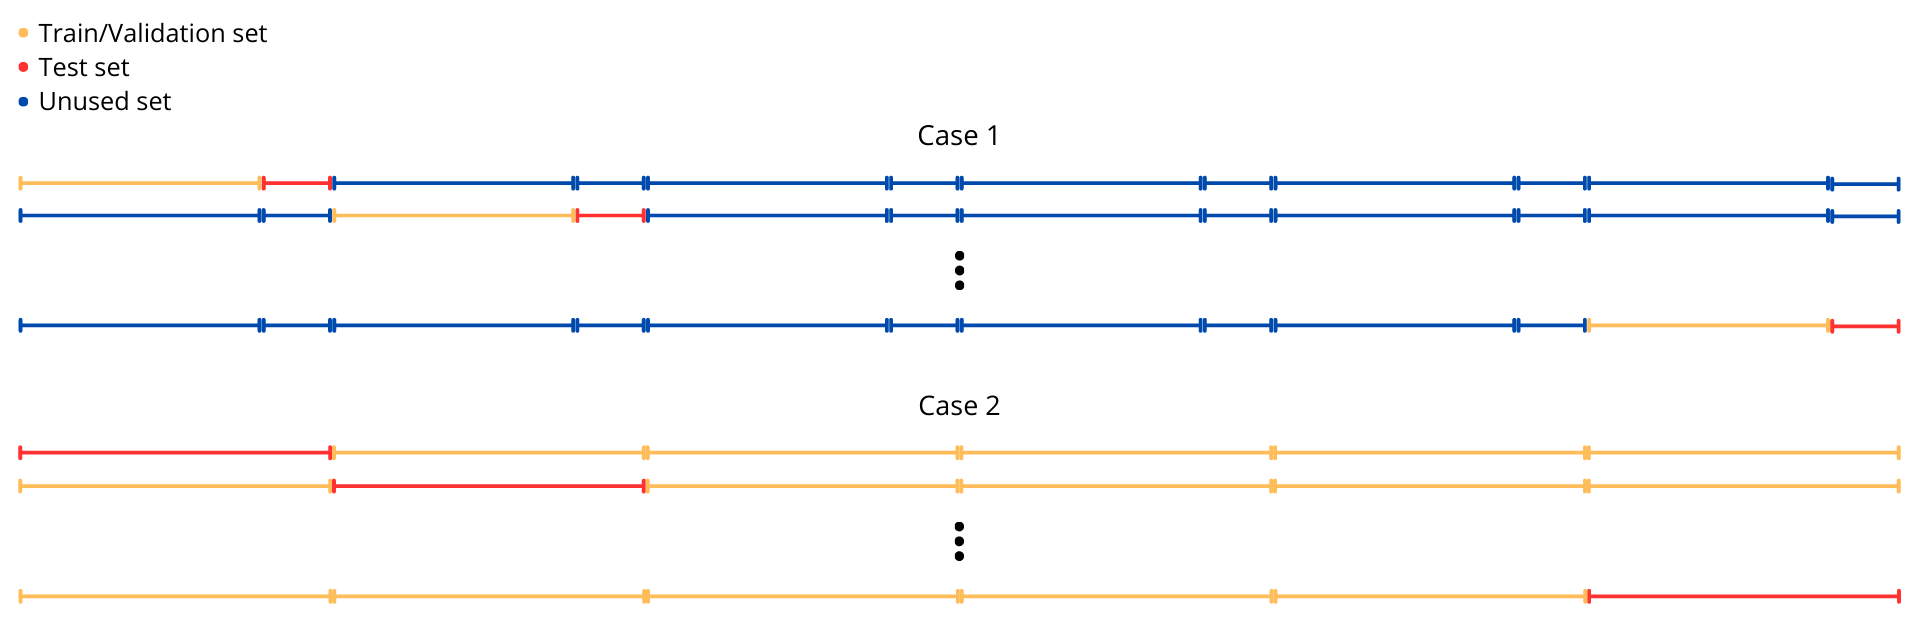
\includegraphics[width=0.98\textwidth]{Canva/datasplits.png}
    \caption{Two cross-validation cases are shown, where the orange region represents the train and validation set, the red region represents the test set, and the blue region is unused for evaluation.
    In \textbf{Case 1}, the dataset is split into six equal-sized folds sorted by date.
    For the selected fold, the last part (colored red) is used for testing, and the remaining part (colored orange) is used for training and validation.
    This process is repeated six times, once for each fold.
    In \textbf{Case 2}, the dataset is again split into six equal-sized folds sorted by date.
    However, this time, one whole fold is used for testing, and the remaining five folds are used for training and validation.
    This process is repeated six times, with each fold used exactly once for testing.}
    \label{fig:datasplit_cases}
\end{figure}




\subsection{Feature Selection}
We trained models using a range of features, specifically $k=[2,5,10,20,30,40,50]$ features.
For each model, we selected the $k$ features that had the greatest mutual information with the target value.
This approach helps us identify the most important features and can improve the model's performance by reducing overfitting and noise.
By selecting different numbers of features, we can explore the trade-off between model complexity and performance.\textcolor{red}{write and ref to mutual info in theory section}.

\subsection{Model Architecture}
We performed a Bayesian hyperparameter search for each model using the parameter space in Table \ref{tab:xgb_hyperparameters_pcorr}.
The search space includes eight hyperparameters that affect the model's complexity, such as the maximum depth of the trees, the regularization strength, and the learning rate.
We used a uniform or log-uniform distribution to sample each hyperparameter within a specific range.
We evaluated $200$ different combinations of hyperparameters (for each dataset, cross-validation case, target variable, and the number of features selected) to find the optimal values for each model.
The models were validated using the MSE, and we picked the model with the best performance on the validation set.


\begin{table}[H]
    \centering
    \caption{This table presents a list of parameters that are sampled during hyperparameter tuning for the pointing correction model. The table includes names, distributions that are sampled from, and corresponding ranges.}
    \begin{tabular}{lcc}
        \hline
        \textbf{Parameter} & \textbf{Sample Distribution} & \textbf{Range} \\ \hline
        max depth & Uniform & [1, 5] \\ 
        reg lambda & Uniform & [0, 1] \\ 
        colsample bytree & Uniform & [0.5, 1] \\ 
        n estimators & Uniform & [20, 500] \\ 
        learning rate & Log-Uniform & [$10^{-5}$, 1] \\ 
        subsample & Uniform & [0.5, 1] \\ 
        gamma & Log-Uniform & [$10^{-5}$, 1] \\ 
        min child weight & Uniform & [1, 10] \\ 
        \hline
    \end{tabular}
    \label{tab:xgb_hyperparameters_pcorr}
\end{table}



\subsection{Model Evaluation}
To evaluate the performance of the models, we calculated the RMS on each test fold and compared it to the current RMS of the telescope on the same data.
The RMS is calculated for azimuth and elevation separately since an XGBoost model only can predict one target.
For a fold $j$ and target either azimuth or elevation, the RMS is calculated by
\begin{equation}
    RMS_{\text{target},j} = \sqrt{\frac{1}{N_j}\sum_{i=1}^{N_j} (\tilde{\delta}_{\text{target},ji} - \delta_{\text{target},ji})^2},
\end{equation}
where $\tilde{\delta}_{\text{target},ji}$ is the predicted pointing offset and $\delta_{\text{target},ji}$ is the true pointing offset for the $i$th pointing scan in fold $j$.
$N_j$ is the number of pointing scans in fold $j$. 
We then computed the ratio $r_{RMS,j}$ of the model's RMS to the current RMS for each fold.
If the ratio is less than $1$, it indicates that the XGBoost model provides an improvement over the current performance of the telescope for a given fold.

To obtain an overall measure of the model's performance compared to the current performance of the telescope, we averaged the ratios $r_{RMS,j}$ over all six test folds
\begin{equation}
    \bar{r}_{RMS} = \sum_{i=1}^6 \frac{RMS_{model,j}}{RMS_{current,j}}.
\end{equation}
This gives us an average ratio $\bar{r}_{RMS}$, which is a measure of the improvement in performance provided by the XGBoost model.
If $\bar{r}_{RMS} < 1$, it indicates that the XGBoost model outperforms the current pointing correction method on average across all test folds.
By comparing the average ratio $\bar{r}_{RMS}$ for the two different cross-validation cases in figure \ref{fig:datasplit_cases} and the selected number of features,
we can identify which models provide the best performance.
